\chapter{Team 1 Agent Design}

\section{Core Idea}
Team 1 Agent was designed around the idea that the agent wants the whole archipelago to survive. However, the agent does have different configurations that allows it to be more malicious than intended such that interesting simulations may occur.

\section{Opinions on Islands}
For an agent to become self-organising, the agent must determine certain actions given a condition without external input. For this to be possible, the agent must have defined conditions which team 1 calls 'emotional state', and hold an opinion about other islands. This will form a basis for the agent to decide on an action.

Initially, the opinion on all existing islands are neutral. Overtime through IITO and IIGO, the opinions on islands will change. This will affect the outcome of IITO and IIGO results. As a note, positive values correspond to positive opinions while negative values correspond to negative opinions.

An agent's emotional state can change depending on the current resources. Below is an example of how an agent's emotional state can be formed:
\begin{itemize}
    \item If current resources > 10 * living cost, the agent is happy.
    \item If 3 * living cost < current resources < 10 * living cost, the agent is anxious.
    \item If the current resources < 3 * living cost, the agent is desperate.
\end{itemize}
The upper and lower bounds can be changed before a game starts. 

\section{IITO Gifts}
During IITO, the agent's opinion of other island is affected. For every gift received, the agent's opinion of the gifter increases. However, the agent's opinion of an island can decrease if that island promised a gift and was not able to fulfil it. 

When team 1 agent receives a request for gifts, the agent will decide how much to offer depending on the agent's current emotional state and the opinion of that island. 

\begin{table} [htb]
    \centering
    \begin{tabular}{|c|p{0.5\textwidth}|}
        \hline
        Emotional State & How is IITO handled? \\
        \hline
        Happy & Agent will give away its resources that satisfies the requested amount. \\
        \hline
        Anxious & Agent will give away a ratio of the requested amount and its current resources. \\
        \hline
        Desperate & Agent will refuse any gift requests that it receives. \\ 
        \hline
    \end{tabular}
\end{table}

Moreover, if the agent's opinion of an island is very high, the agent can decide to give gifts disregarding the agent's own anxiety. On the other hand, if an opinion of an island is very low, the agent can decide to refuse to send a gift even though the agent is happy. 

For increase survivability, team 1 agent will accept any gift offers that it receives. 

\subsection{Future Works}
Team 1 agent currently has a very straight-forward IITO strategy. Some interesting alteration to this strategy could include:
\begin{itemize}
    \item Being less suspectible to bribery. The agent should stop increasing the opinion of an island after receiving $X$ amount of continuous gifts.
    \item Stop handing out gifts to islands that are not in critical state.
    \item Being proactive in bribery. The agent will give unrequested gifts to the current president in hopes that this will reduce tax and increase resource allocation from the common pool. 
\end{itemize}

\section{IIFO Disaster Prediction}
Disasters can happen deterministically or stochastically (mentioned in detail in Chapter~\ref{sec: Disaster} for more information). For an agent, it is important to determine when a disaster occurs so that as much disaster damage is mitigated using the common pool. 

When the game starts, the disaster prediction made by the agent is random. This prediction always has a confidence value of 0. As more disasters occur, a history of disasters is built up. Using this history, the mean disaster position x, position y, magnitude and occurrence is calculated. A confidence value is calculated along with the mean disaster metrics. 

% Add a footnote on website?  https://www.mathsisfun.com/data/confidence-interval.html
The confidence value is calculated by finding the ratio between margin of error and the mean value. The smaller the margin of error, the more confident the agent is. Therefore, a difference between the mean value and the margin of error must also be calculated. To begin with, the agent uses the confidence interval equation (where $s =$ standard deviation, $n = $ size of array, $Z = $ confidence interval) to calculate the margin of error:
\begin{equation}
    \label{eq: Team1MarginOfError}
    \text{Error} = Z \dfrac{s}{\sqrt{n}} 
\end{equation}
Using the difference between the mean value ($\bar{x}$) and the margin of error along with finding out the ratio of this result will provide the agent with the confidence value.
\begin{equation}
    \text{Confidence Value} = (\bar{x} - \text{Error}) \times \dfrac{1}{\bar{x}}
\end{equation}

Sharing and obtaining other disaster information to and from other islands respectively can increase the survivability of the archipelago. As more disaster prediction is shared, a network of trust between team 1 agent and other island is built. This trust value is primarily based upon the absolute value of the islands prediction on the day the disaster happened. However, if an island shares a disaster prediction with the estimated disaster day to be random or changing erratically each turn, then team 1 agent will begin to distrust that island. 

\section{IIGO: President}

\section{Foraging}
Multiple foraging strategies were developed: 
\begin{itemize}
    \item Return on Investment (ROI)
    \item Regression
    \item Flip Forage
\end{itemize}

Multiple foraging strategies were developed, initially by intuition and later by attempting to address the shortcomings of previous attempts.

\subsection{Return on Investment (ROI) Foraging}%
\label{sec:forage-roi}

This first algorithm is based on repeating successful foraging behaviours in the past, whether those be by the agent herself or another agent.

For the first few turns (the exact amount is configurable) the agent will forage randomly.

The agent maintains a history of foraging decisions and outcomes, including those received from IIFO.\@ When it comes time to forage this history is sorted by ROI, i.e.\ the ratio of profit to contribution. Decisions that resulted in a loss, had profit smaller that the living cost, or had a larger contribution that a (configurable) percentage of available resources are filtered out.

\subsection{Regression Foraging}%
\label{sec:forage-regression}

This strategy tries to predict the ideal foraging decision, even if that exact decision was not made in the past. This is done using regression, which is used to find the decision with the highest expected reward.

% In detail, history is kept as in \nameref{sec:forage-roi}. To make a foraging decision, the history is split by foraged resource (fish or deer), and quadratic regression is performed on contribution versus reward. The maximum of the regression curve is found for each group and the contribution with the highest

\subsection{Flip Foraging}

This strategy chooses the least foraged resource from the last turn, according to IIFO-reported data. Contributed amount is proportional to the chosen resource's total ROI from last turn. This choice was made under the assumption that ROI is an indicator of the resource's ``condition''. If a resource only gives moderate rewards (proportionally to input) it means that it is probably over-used currently and as such agents should allow it to recover, by scaling down their foraging attempts.

\subsection{Comparison}

To compare the three strategies, simulations were run with six agents, two using \emph{ROI foraging}, two using \emph{regression foraging}, and two using \emph{flip foraging}. IIGO and IITO were also disabled in order to isolate the efficacy of foraging methods from other parts of the game. The simulation was run five times and the results averaged over the 5 games as well as the two agents following the same strategy.

\begin{figure}[H] 
\centering
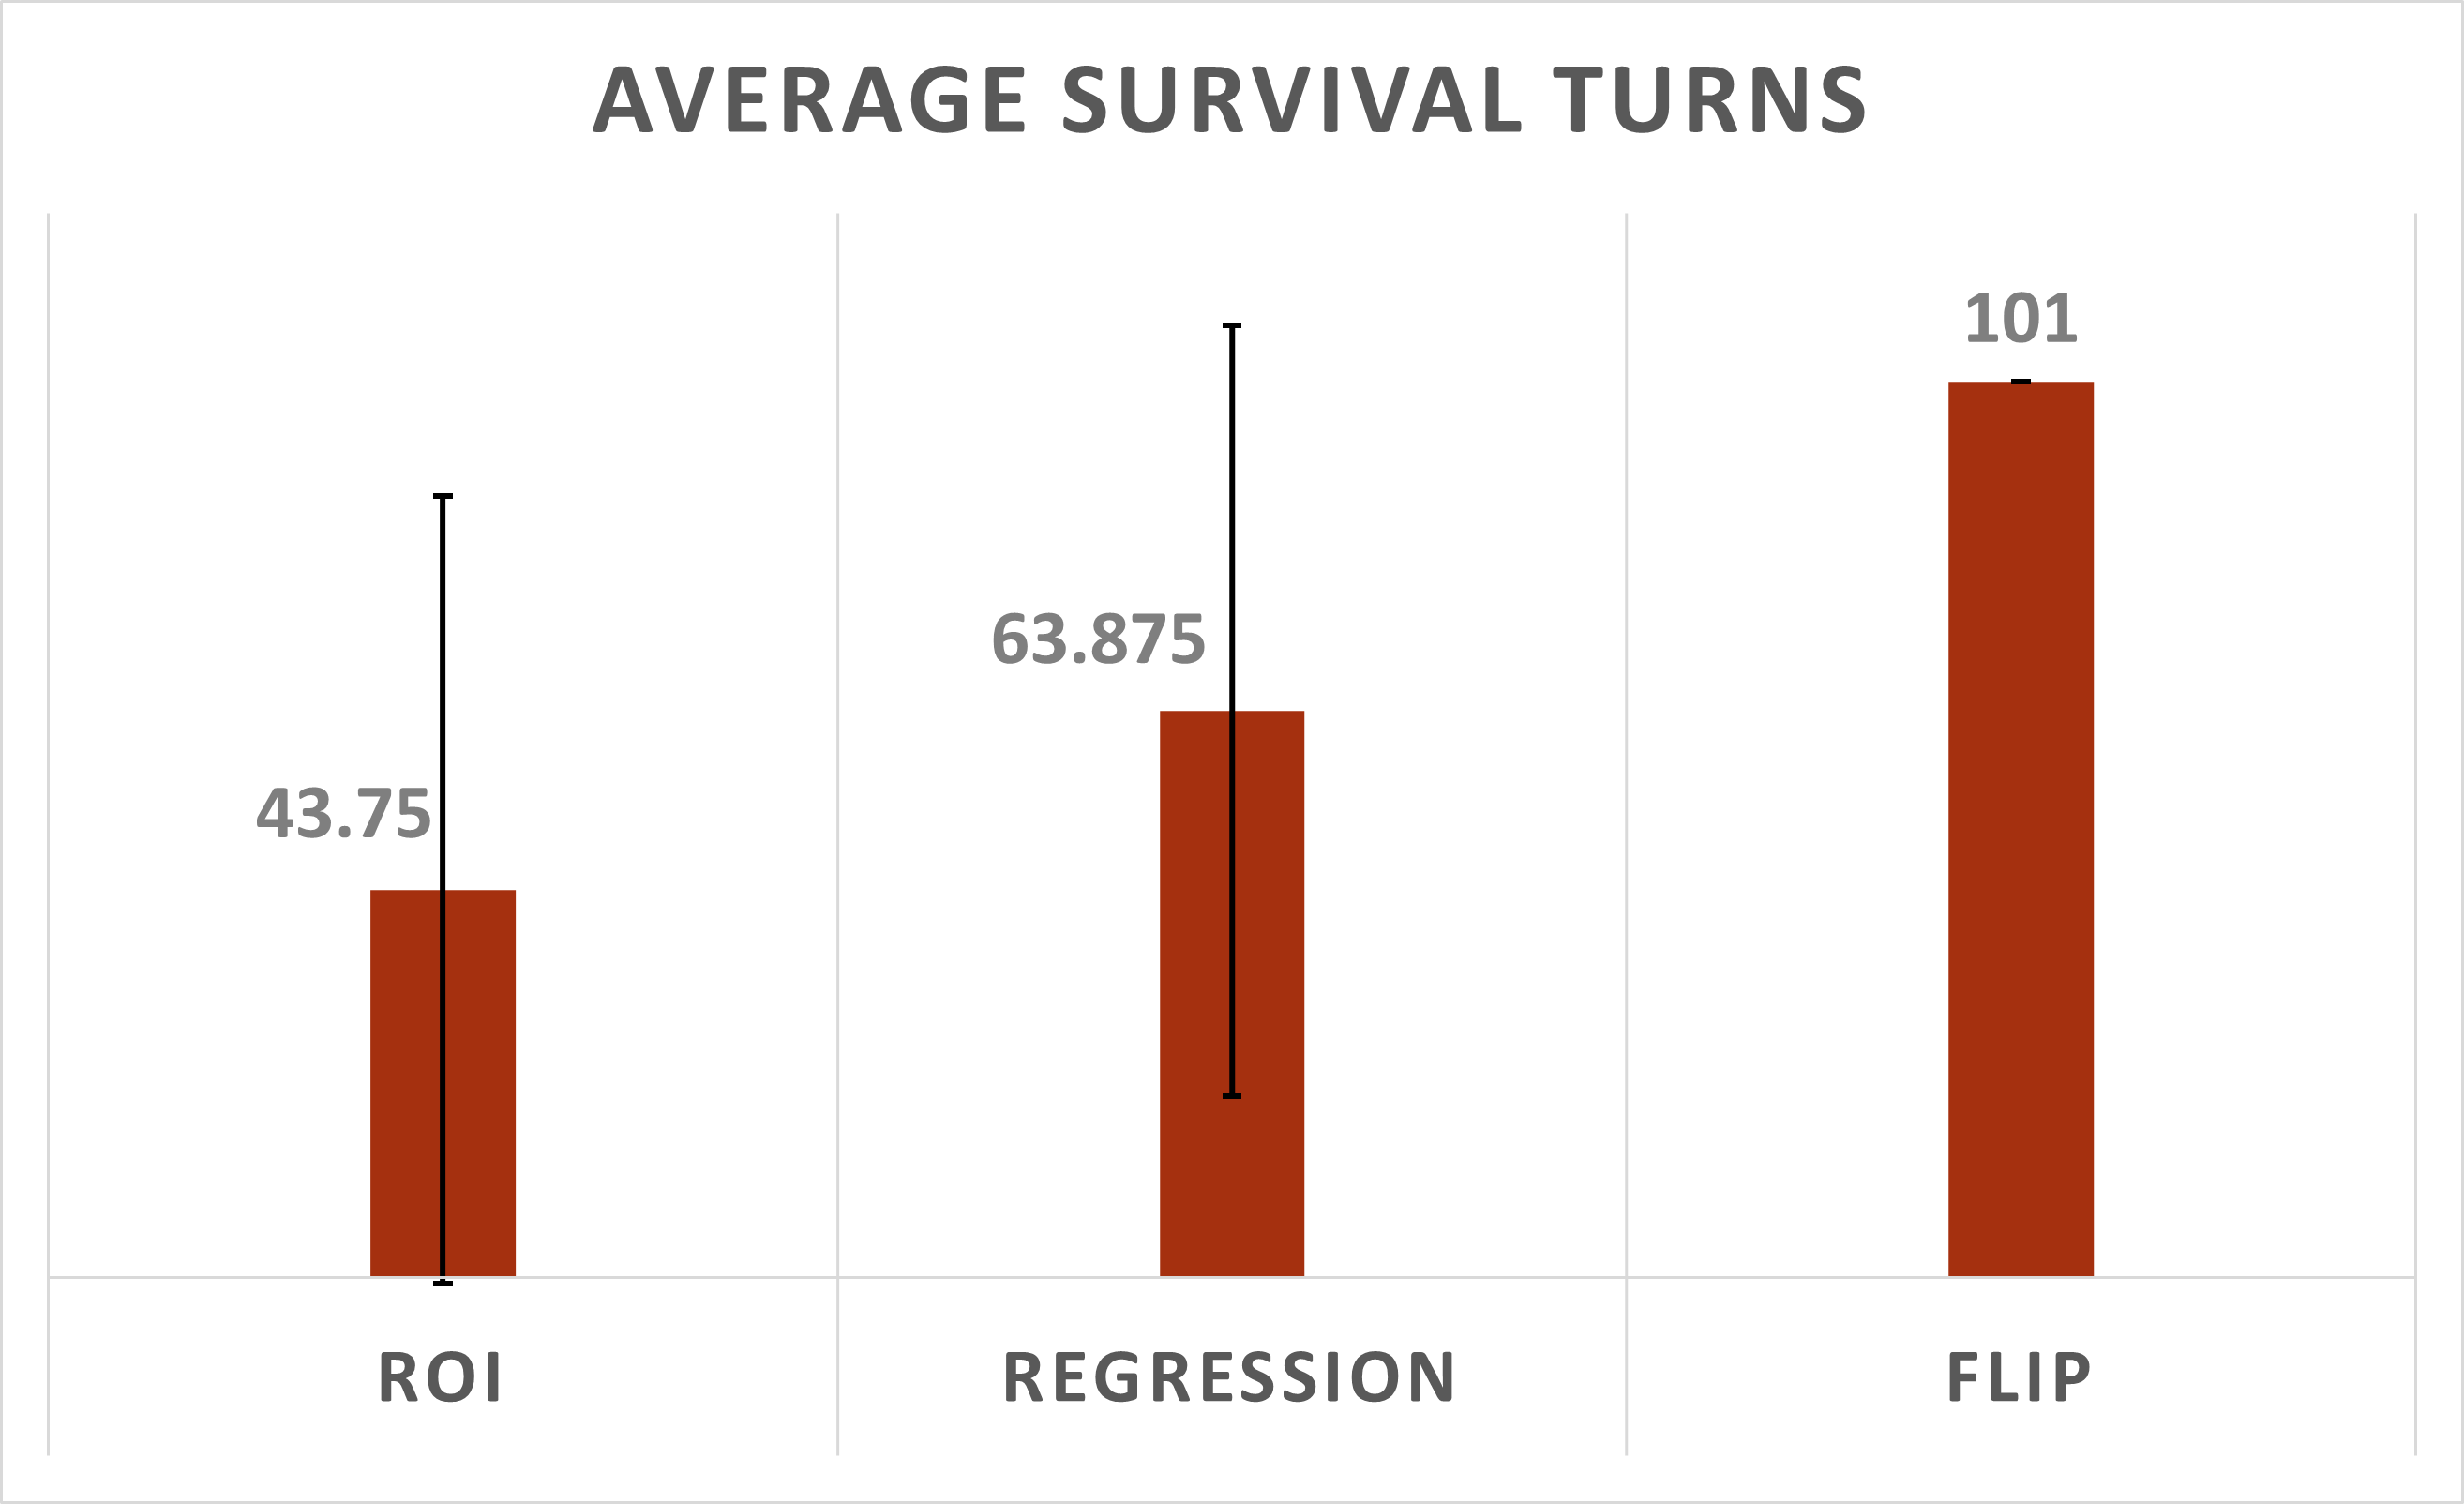
\includegraphics[width=0.6\textwidth]{09_team1_agentdesign/images/mean_survival_turns}
\caption{Mean survival turns for different strategies.}
\label{fig:team1:mean_survival}
\end{figure} 

\begin{figure}[H] 
\centering
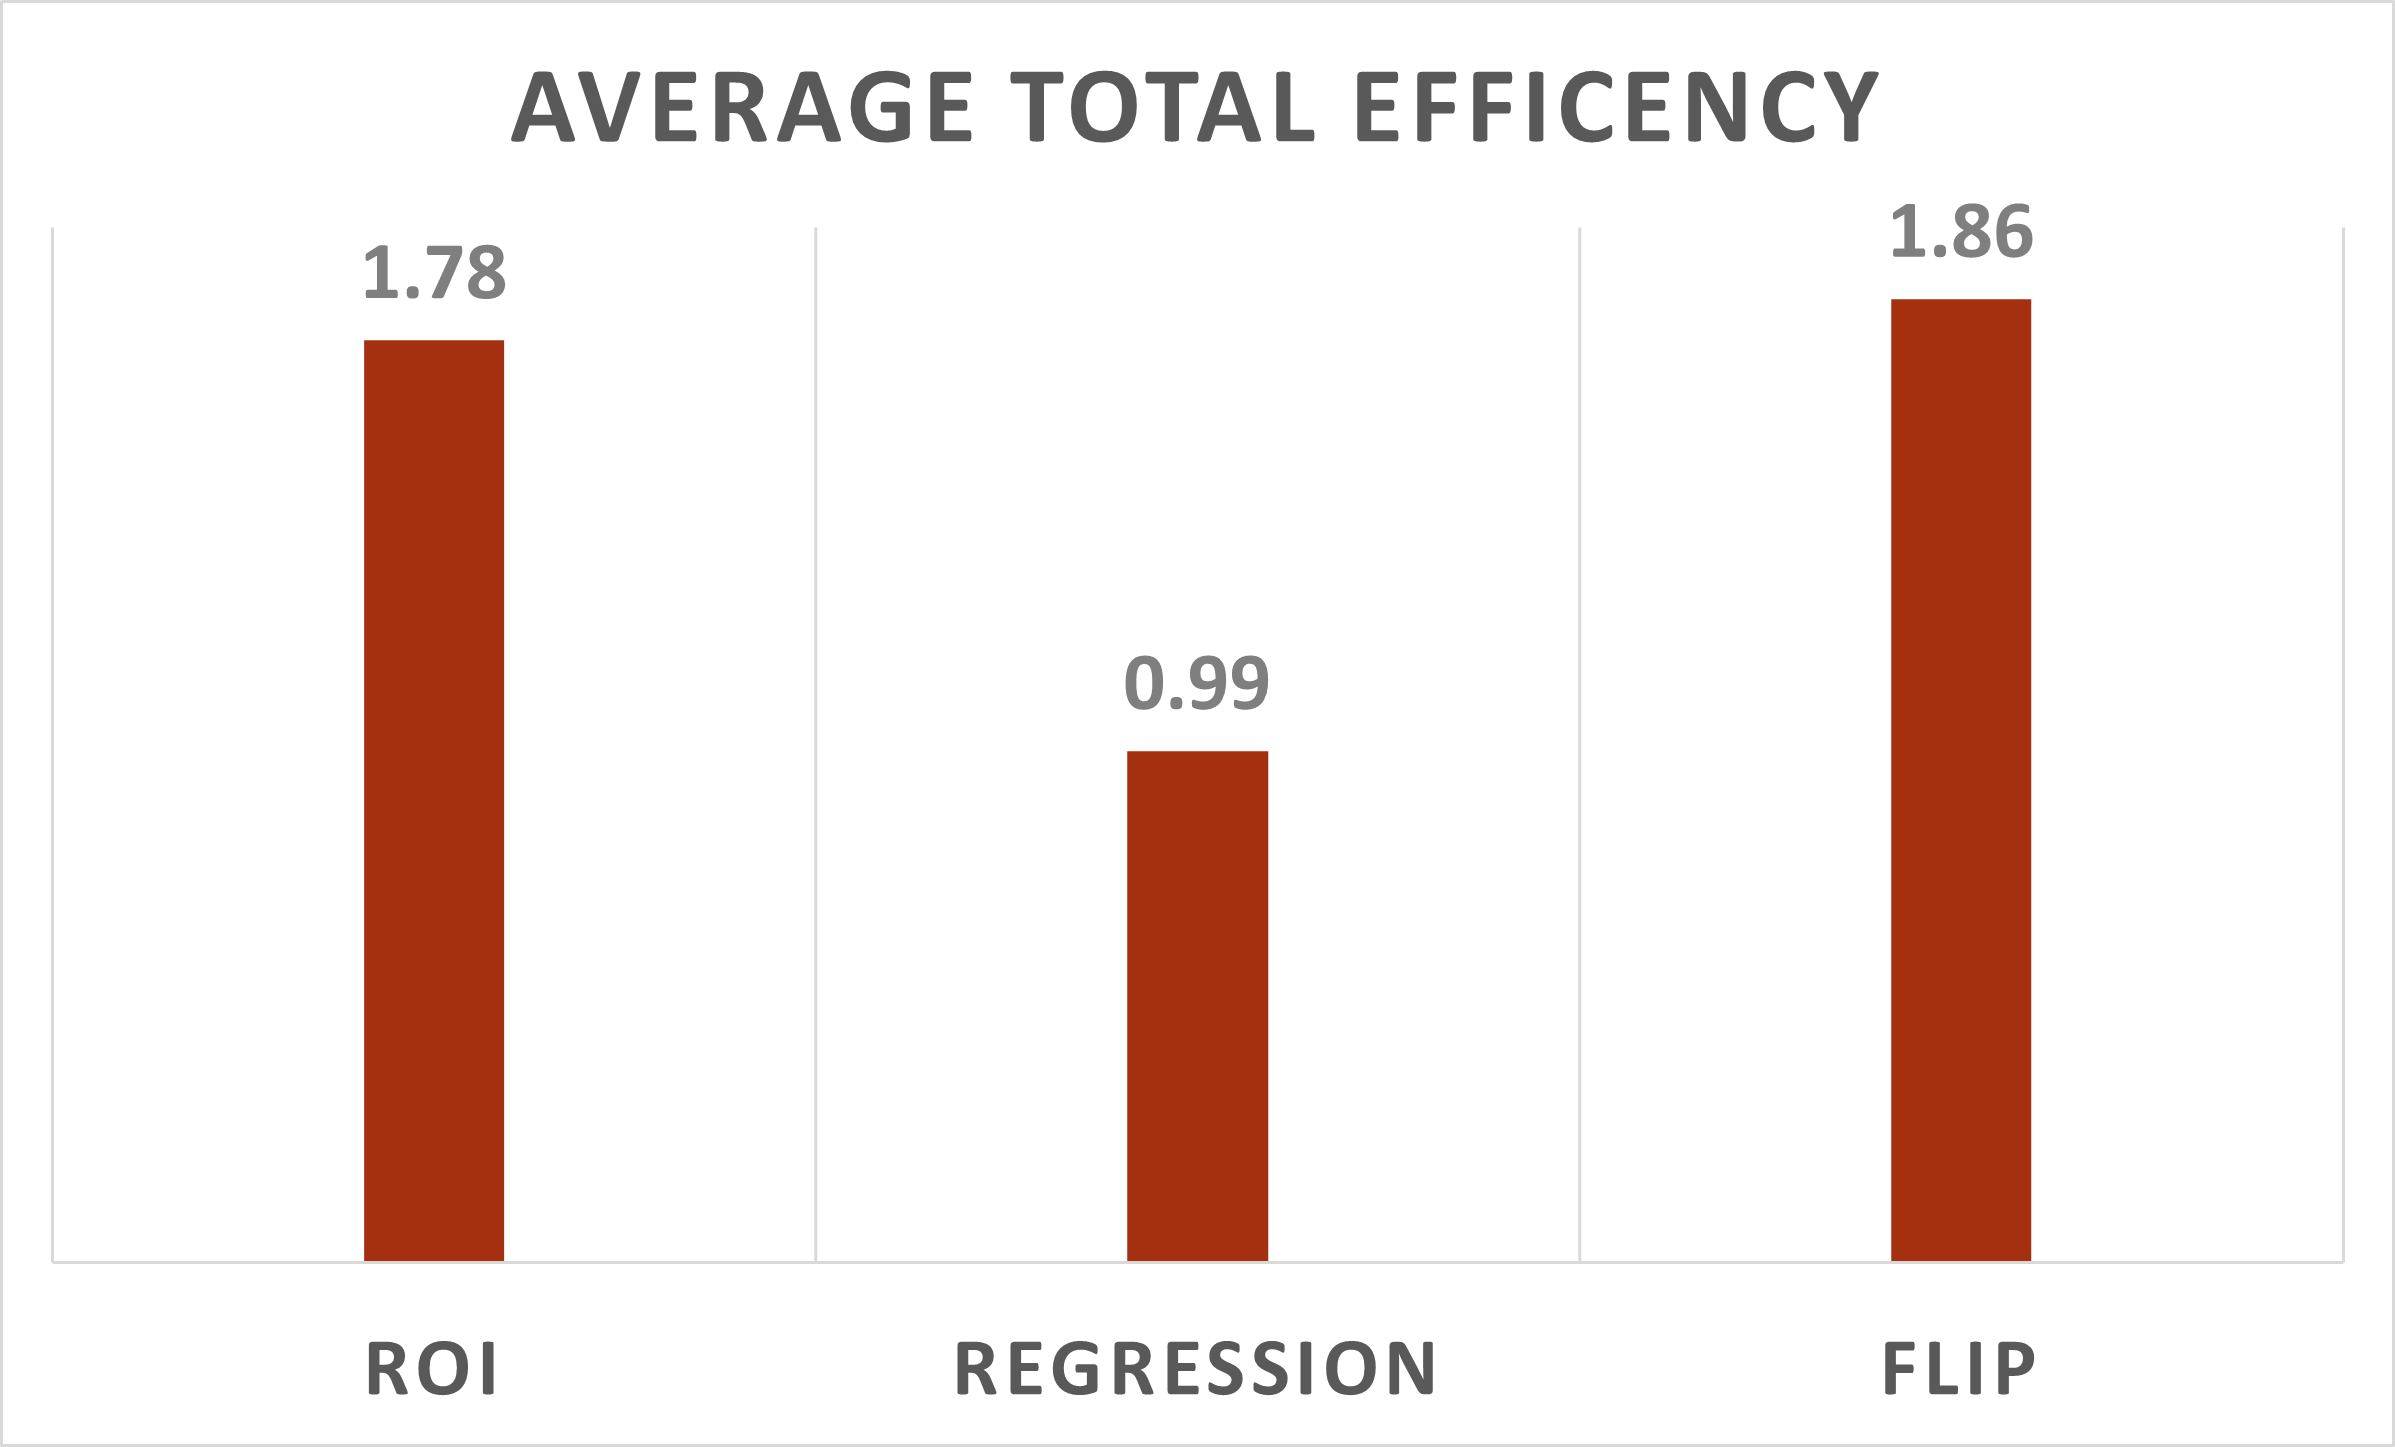
\includegraphics[width=0.6\textwidth]{09_team1_agentdesign/images/total_efficiency}
\caption{Average foraging efficiency}
\label{fig:team1:average_efficiency}
\end{figure} 

It is clear from \autoref{fig:team1:mean_survival} that the \emph{flip} foraging strategy dominates the other two in terms of overall effectiveness. However, it is interesting to note that, according to \autoref{fig:team1:average_efficiency}, the \emph{ROI} foraging method is almost as efficient as \emph{flip}, which raises the question of what causes the difference in their success. This difference could be attributed to one core issue with the \emph{ROI strategy}: ignoring the absolute value of rewards. The agent will happily settle for a profit of $11$ resources, if that was obtained with a contribution of $0.1$ resources (a profit of $110000\%$) over a profit $50$ resources for a contribution of $25$ (a measly $100\%$). This means that in the long run living costs overwhelm the \emph{ROI} agent. The \emph{flip} agent does not take expected profit into account and as such is unaffected by this.

\emph{Regression} appears to occupy a medium between \emph{flip} and \emph{ROI}, however it is much less consistent, as evidenced by the error bars in \autoref{fig:team1:mean_survival}, with \emph{regression} surviving for under 10 turns in some runs.

%%% Local Variables:
%%% mode: latex
%%% TeX-master: "../main"
%%% End:
